
\documentclass[letterpaper, 11pt]{article}
\usepackage[utf8]{inputenc}
\usepackage{titlesec}
\usepackage{fullpage} % changes the margin
\usepackage{graphicx} %package to manage images
\usepackage{tabularx}
\graphicspath{ {./images/} }

\begin{document}
\begin{titlepage}
\vspace*{0.7in}
\begin{center}
\begin{figure}[htb]
\begin{center}

\includegraphics[width=8cm]{univ_logo}
\end{center}
\end{figure}
\vspace*{0.3in}
\begin{Large}
\textbf{SOEN 6011 : SOFTWARE ENGINEERING PROCESSES} \\
\end{Large}
\vspace*{0.1in}
\begin{Large}
\textbf{SUMMER 2022} \\
\end{Large}
\vspace*{0.9in}
\begin{Large}
\textbf{ETERNITY} \\
\end{Large}
\vspace*{0.9in}
\begin{Large} 


\textbf{PROBLEM - 5} \\
Unit Test cases \\
\end{Large}
\vspace*{0.625in}
\rule{80mm}{0.1mm}\\
\vspace*{0.1in}
\begin{large}
Author \\
\vspace*{0.1in}
Neona Sheetal Pinto\\
\vspace*{1.0in}
\date{\normalsize\today} 
\end{large}
\end{center}
\begin{center}
https://www.overleaf.com/project/62ed25babfddf15056d6b5f7\end{center}
\end{titlepage}
\tableofcontents
\listoffigures
\newpage
\section{{PROBLEM 7 - F6: $B(x,y)$}}
    \subsection{Test cases of F6 $B(x,y)$}
    As per Java coding standards, the JUnit test cases are created and maintained in a separate folder structure to perform the testing process with zero impact on code section as shown in figure \ref{fig:test_org} \\
    \subsection{Test Environment}
        \begin{itemize}
            \item IntelliJ IDE for Java
            \item  JUnit4 framework in IntelliJ IDE for
            testing(4.12) shown in figure 
        \end{itemize}

    \subsection{Testing steps}
        \begin{itemize}
            \item Build and Compile the F6 function code in IntelliJ.
            \item On successful compilation run the F6 function.
            \item Give different inputs according to the requirements(R2)
            \item Run the JUnit4 for all the test classes to check the output
            \item Run all the test cases uses the Test suite, making sure all the test cases are successful.
            \item Verify the output as shown in figure \ref{fig:junit}
        \end{itemize}
    \subsection{Test cases}
        \subsubsection{\textbf{Test case 1:}} 
            \setlength{\tabcolsep}{25pt}
            \renewcommand{\arraystretch}{1.5}
            \begin{tabularx}{1.0\textwidth} { 
                  | >{\raggedright\arraybackslash}X 
                  | >{\raggedright\arraybackslash}X | }
                 \hline
                 Function & testBetaFunctionWithPositiveValues()\\
                 \hline
                 Input  & BetaFunction(3,4) , 0.001)\\
                  \hline
                 Expected  & 0.0166667\\
                  \hline
                 Result  & Passed\\
                  \hline
                 Requirement ID  & R1\\
                   \hline
                 Comment  & Testing the Beta function with 2 positive values using assertEquals and comparing expected and actual value\\
                \hline
            \end{tabularx}
        \subsubsection{\textbf{Test case 2:}} 
            \setlength{\tabcolsep}{25pt}
            \renewcommand{\arraystretch}{1.5}
            \begin{tabularx}{1.0\textwidth} { 
                  | >{\raggedright\arraybackslash}X 
                  | >{\raggedright\arraybackslash}X | }
                 \hline
                 Function & testBetaFunctionWithNegativeValues()\\
                 \hline
                 Input  & BetaFunction(-3.4,-4.5)\\
                  \hline
                 Expected  & -1\\
                  \hline
                 Result  & Passed\\
                  \hline
                 Requirement ID  & R1\\
                    \hline
                 Comment  & Testing the Beta function with 2 negative values using assertEquals and comparing expected and actual value\\
                \hline
            \end{tabularx} 
        \subsubsection{\textbf{Test case 3:}}  
            \setlength{\tabcolsep}{25pt}
            \renewcommand{\arraystretch}{1.5}
            \begin{tabularx}{1.0\textwidth} { 
                  | >{\raggedright\arraybackslash}X 
                  | >{\raggedright\arraybackslash}X | }
                 \hline
                 Function & testBetaFunctionWithOneNegativeValues()\\
                 \hline
                 Input  & BetaFunction(-3.4,4.5)\\
                  \hline
                 Expected  & -1\\
                  \hline
                 Result  & Passed\\
                  \hline
                 Requirement ID  & R1\\
                    \hline
                 Comment  & Testing the Beta function with one negative values using assertEquals and comparing expected and actual value\\
                \hline
            \end{tabularx} 

        \subsubsection{\textbf{Test case 4:}}  
            \setlength{\tabcolsep}{25pt}
            \renewcommand{\arraystretch}{1.5}
            \begin{tabularx}{1.0\textwidth} { 
                  | >{\raggedright\arraybackslash}X 
                  | >{\raggedright\arraybackslash}X | }
                 \hline
                 Function & testBetaFunctionWithZeroValues()\\
                 \hline
                 Input  & BetaFunction(0,0)\\
                  \hline
                 Expected  & -1\\
                  \hline
                 Result  & Passed\\
                  \hline
                 Requirement ID  & R1\\
                    \hline
                 Comment  & Testing the Beta function with zero values using assertEquals and comparing expected and actual value\\
                \hline
            \end{tabularx} 

        \subsubsection{\textbf{Test case 5:}} 
            \setlength{\tabcolsep}{25pt}
            \renewcommand{\arraystretch}{1.5}
                \begin{tabularx}{1.0\textwidth} { 
                  | >{\raggedright\arraybackslash}X 
                  | >{\raggedright\arraybackslash}X | }
                 \hline
                 Function & testBetaFunctionWithIntegralFunction()\\
                 \hline
                 Input  & integral(0, 1, 3.4, 4.5, (x1, p, q) -$>$ (exp.calculateResult(x1, (p - 1))) * (exp.calculateResult((1- x1), (q-1)))), 0.001)\\
                  \hline
                 Expected  & 0.0084110\\
                  \hline
                 Result  & Passed\\
                  \hline
                 Requirement ID  & R1\\
                    \hline
                 Comment  & Testing the Beta function along with Integral function with double values using assertEquals and comparing expected and actual value\\
                \hline
            \end{tabularx} 
        \subsubsection{\textbf{Test case 6:}} 
            \setlength{\tabcolsep}{25pt}
            \renewcommand{\arraystretch}{1.5}
            \begin{tabularx}{1.0\textwidth} { 
                  | >{\raggedright\arraybackslash}X 
                  | >{\raggedright\arraybackslash}X | }
                 \hline
                 Function & positiveNumberPowerofPositiveNumber()\\
                 \hline
                 Input  & calculateResult(5, 9)\\
                  \hline
                 Expected  & Math.pow(5,9)\\
                  \hline
                 Result  & Passed\\
                  \hline
                 Requirement ID  & R3\\
                    \hline
                 Comment  & Testing the Exponent function used in the Beta function along with positive values using assertEquals and comparing expected and actual value. The expected value is computed using Math function to check the accuracy.\\
                \hline
            \end{tabularx} 

        \subsubsection{\textbf{Test case 7:}} 
            \setlength{\tabcolsep}{25pt}
            \renewcommand{\arraystretch}{1.5}
            \begin{tabularx}{1.0\textwidth} { 
                  | >{\raggedright\arraybackslash}X 
                  | >{\raggedright\arraybackslash}X | }
                 \hline
                 Function & zeroPowerofZero()\\
                 \hline
                 Input  & calculateResult(0, 0)\\
                  \hline
                 Expected  & Math.pow(0,0)\\
                  \hline
                 Result  & Passed\\
                  \hline
                 Requirement ID  & R3\\
                    \hline
                 Comment  & Testing the Exponent function used in the Beta function along with zero values using assertEquals and comparing expected and actual value. The expected value is computed using Math function to check the accuracy.\\
                \hline
            \end{tabularx} 

        \subsubsection{\textbf{Test case 8:}} 
            \setlength{\tabcolsep}{25pt}
            \renewcommand{\arraystretch}{1.5}
            \begin{tabularx}{1.0\textwidth} { 
                  | >{\raggedright\arraybackslash}X 
                  | >{\raggedright\arraybackslash}X | }
                 \hline
                 Function & zeroPowerofRealNumber()\\
                 \hline
                 Input  & calculateResult(0, 3)\\
                  \hline
                 Expected  & Math.pow(0,3)\\
                  \hline
                 Result  & Passed\\
                  \hline
                 Requirement ID  & R3\\
                    \hline
                 Comment  & Testing the Exponent function used in the Beta function along with zero value as base and real number as power using assertEquals and comparing expected and actual value. The expected value is computed using Math function to check the accuracy.\\
                \hline
            \end{tabularx} 
        \subsubsection{\textbf{Test case 9:}} 
            \setlength{\tabcolsep}{25pt}
            \renewcommand{\arraystretch}{1.5}
            \begin{tabularx}{1.0\textwidth} { 
                  | >{\raggedright\arraybackslash}X 
                  | >{\raggedright\arraybackslash}X | }
                 \hline
                 Function & positiveNumberPowerofZero()\\
                 \hline
                 Input  & calculateResult(7, 0)\\
                  \hline
                 Expected  & Math.pow(7,0)\\
                  \hline
                 Result  & Passed\\
                  \hline
                 Requirement ID  & R3\\
                    \hline
                 Comment  & Testing the Exponent function used in the Beta function along with real value as base and zero as the power using assertEquals and comparing expected and actual value. The expected value is computed using Math function to check the accuracy.\\
                \hline
            \end{tabularx} 
        \subsubsection{\textbf{Test case 10:}} 
            \setlength{\tabcolsep}{25pt}
            \renewcommand{\arraystretch}{1.5}
            \begin{tabularx}{1.0\textwidth} { 
                  | >{\raggedright\arraybackslash}X 
                  | >{\raggedright\arraybackslash}X | }
                 \hline
                 Function & negativeNumberPowerofZero()\\
                 \hline
                 Input  & calculateResult(-4, 0)\\
                  \hline
                 Expected  & Math.pow(-4,0)\\
                  \hline
                 Result  & Passed\\
                  \hline
                 Requirement ID  & R3\\
                    \hline
                 Comment  & Testing the Exponent function used in the Beta function along with real negative value as base and zero as the power using assertEquals and comparing expected and actual value. The expected value is computed using Math function to check the accuracy.\\
                \hline
            \end{tabularx} 
        \subsubsection{\textbf{Test case 11:}} 
            \setlength{\tabcolsep}{25pt}
            \renewcommand{\arraystretch}{1.5}
            \begin{tabularx}{1.0\textwidth} { 
                  | >{\raggedright\arraybackslash}X 
                  | >{\raggedright\arraybackslash}X | }
                 \hline
                 Function & positiveNumberPowerofOne()\\
                 \hline
                 Input  & calculateResult(7, 1)\\
                  \hline
                 Expected  & Math.pow(7,1)\\
                  \hline
                 Result  & Passed\\
                  \hline
                 Requirement ID  & R3\\
                    \hline
                 Comment  & Testing the Exponent function used in the Beta function along with real  value as base and one as the power using assertEquals and comparing expected and actual value. The expected value is computed using Math function to check the accuracy.\\
                \hline
            \end{tabularx} 

        \subsubsection{\textbf{Test case 12:}} 
            \setlength{\tabcolsep}{25pt}
            \renewcommand{\arraystretch}{1.5}
            \begin{tabularx}{1.0\textwidth} { 
                  | >{\raggedright\arraybackslash}X 
                  | >{\raggedright\arraybackslash}X | }
                 \hline
                 Function & numericInputCheckTest()\\
                 \hline
                 Input  & numericInputCheck(12.3, 43)
                 numericInputCheck(0, 0)
                 numericInputCheck(3, 6)
                 numericInputCheck(-43, 89)
                 numericInputCheck(54, -65)
                 numericInputCheck(-54, -56)\\
                  \hline
                 Expected  & True or false based on the inputs\\
                  \hline
                 Result  & Passed\\
                  \hline
                 Requirement ID  & R1 AND R7\\
                    \hline
                 Comment  & Multiple input checks to ensure that the correct inputs are passed to the Beta function.\\
                \hline
            \end{tabularx} 
    \newpage
    \subsection{Snapshots of testing for $B(x,y)$}

        \begin{figure}[htb]
            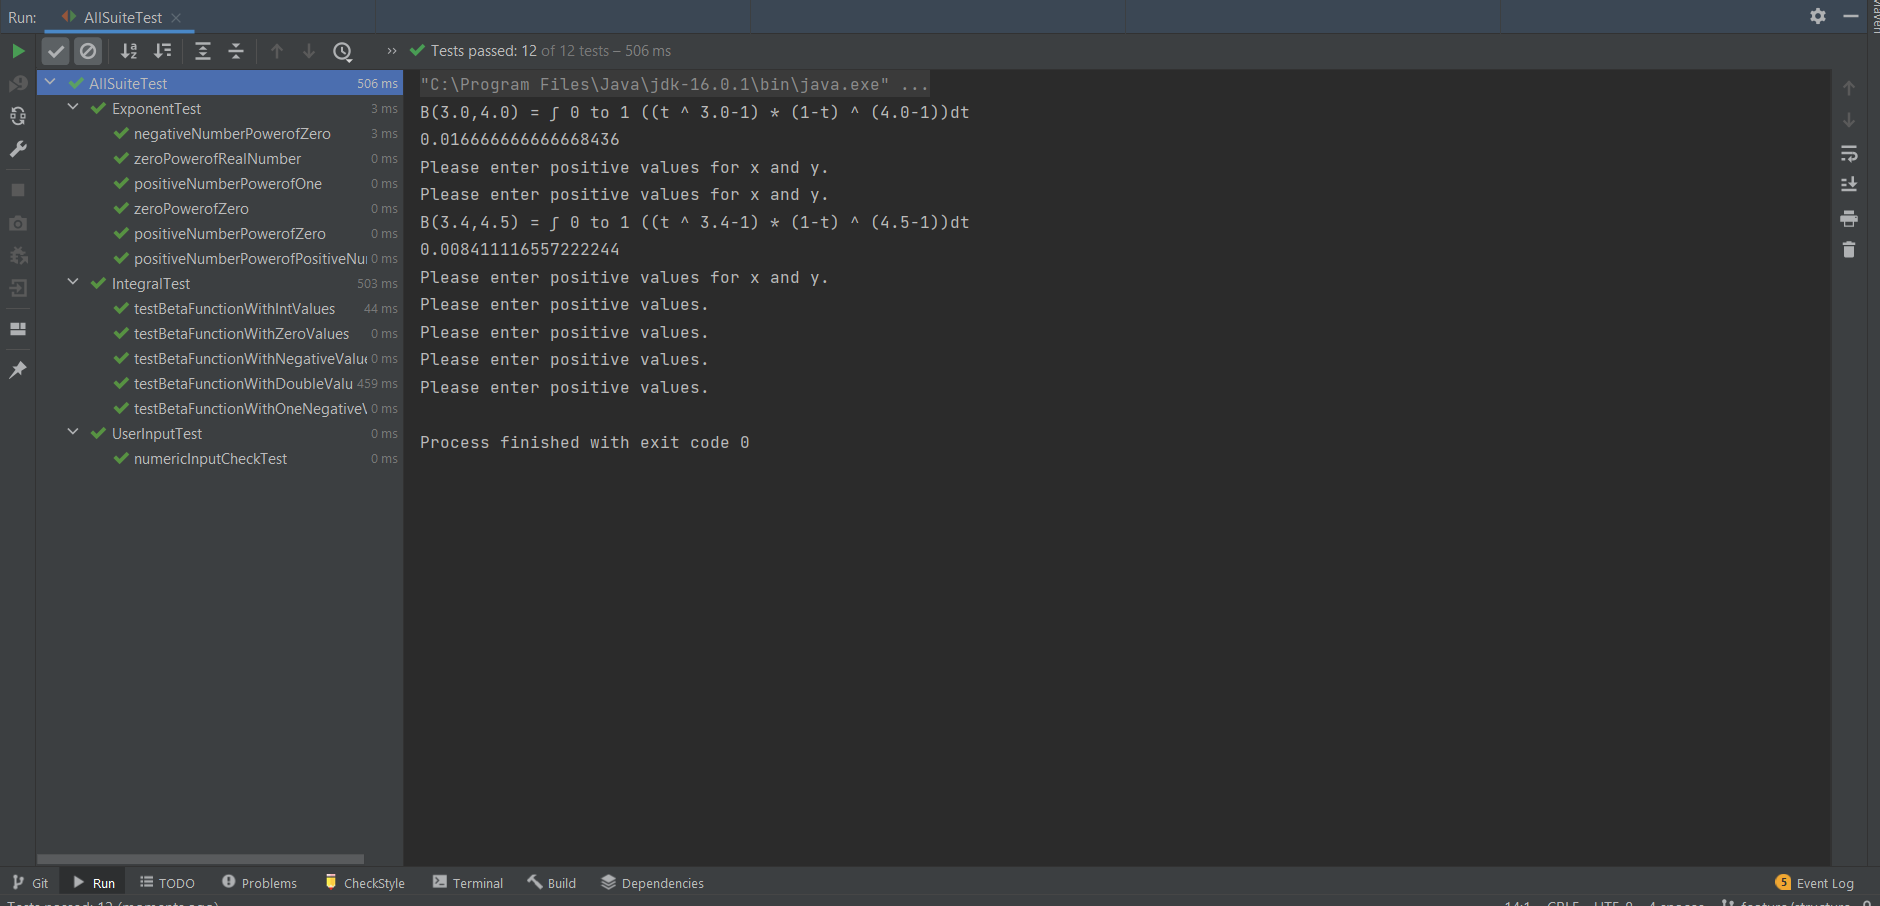
\includegraphics[width=1.1\textwidth]{Testcases.PNG}
            \centering
            \caption{Testing Results Using JUnit-4 All Suite Test for F6 Function}
            \label{fig:junit}
        \end{figure} 
        
        \begin{figure}[htb]
            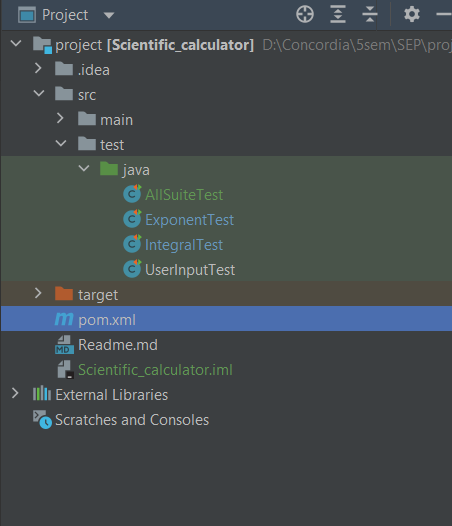
\includegraphics[width=0.5\textwidth]{test_organisation.PNG}
            \centering
            \caption{Separation of code from test cases}
            \label{fig:test_org}
        \end{figure} 

    \subsection{Annexure:}
        \begin{itemize}
          \item \textbf{Trello Board :} \textit{https://trello.com/eternity119}
          \item \textbf{Code Version Control :} \textit{https://github.com/neonapinto/Scientific\_calculator}
          \item \textbf{Overleaf :} \textit{https://www.overleaf.com/project/62ed25babfddf15056d6b5f7}
        \end{itemize}
        
\end{document}